\graphicspath{{pict/}}
\DeclareGraphicsExtensions{.pdf,.png,.jpg}

\chapter{Конструкторский раздел}
\label{cha:design}

В данной работе для нахождения произведения матриц используются алгоритмы стандартный, Винограда и Винограда с оптимизациями. Необходимо рассмотреть и изучить данные варианты реализации.

\section{IDEF0 Модель}

На рисунке 2.1 приведена функциональная модель множения матриц в нотации IDEF0.
\begin{figure}
\centering
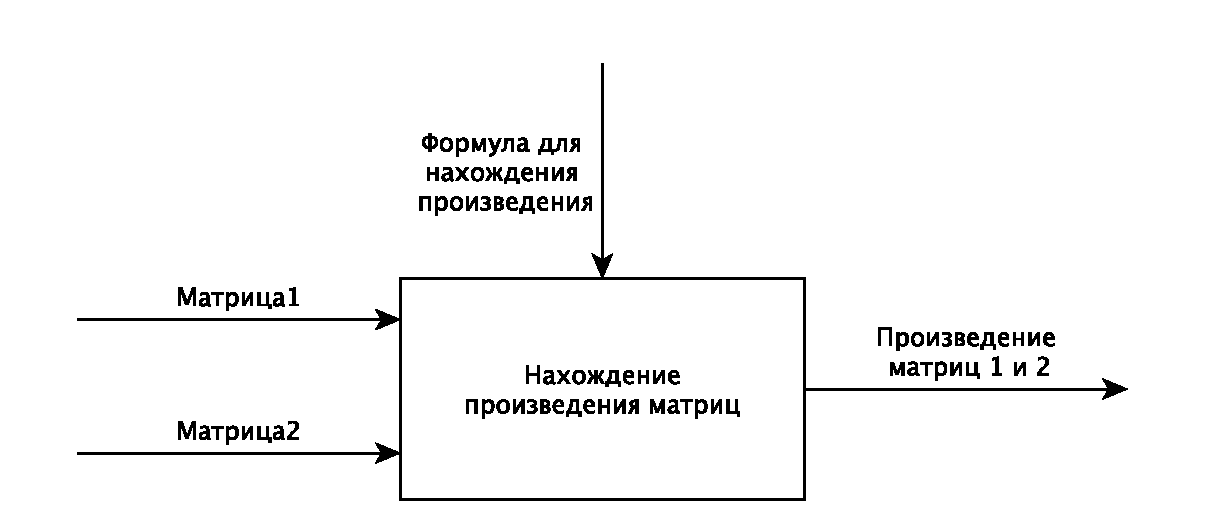
\includegraphics[scale=0.75]{idef0.pdf}
\caption{Функциональная модель умножения матриц}
\end{figure}
\newpage

\section{Разработка алгоритмов}
В данном разделе рассматриваются необходимые алгоритмы с помощью блок-схем.
\subsection{Классический алгоритм умножения матриц}
На рисунке 2.2 представлен стандартный алгоритм перемножения матриц.
\begin{figure}
\centering
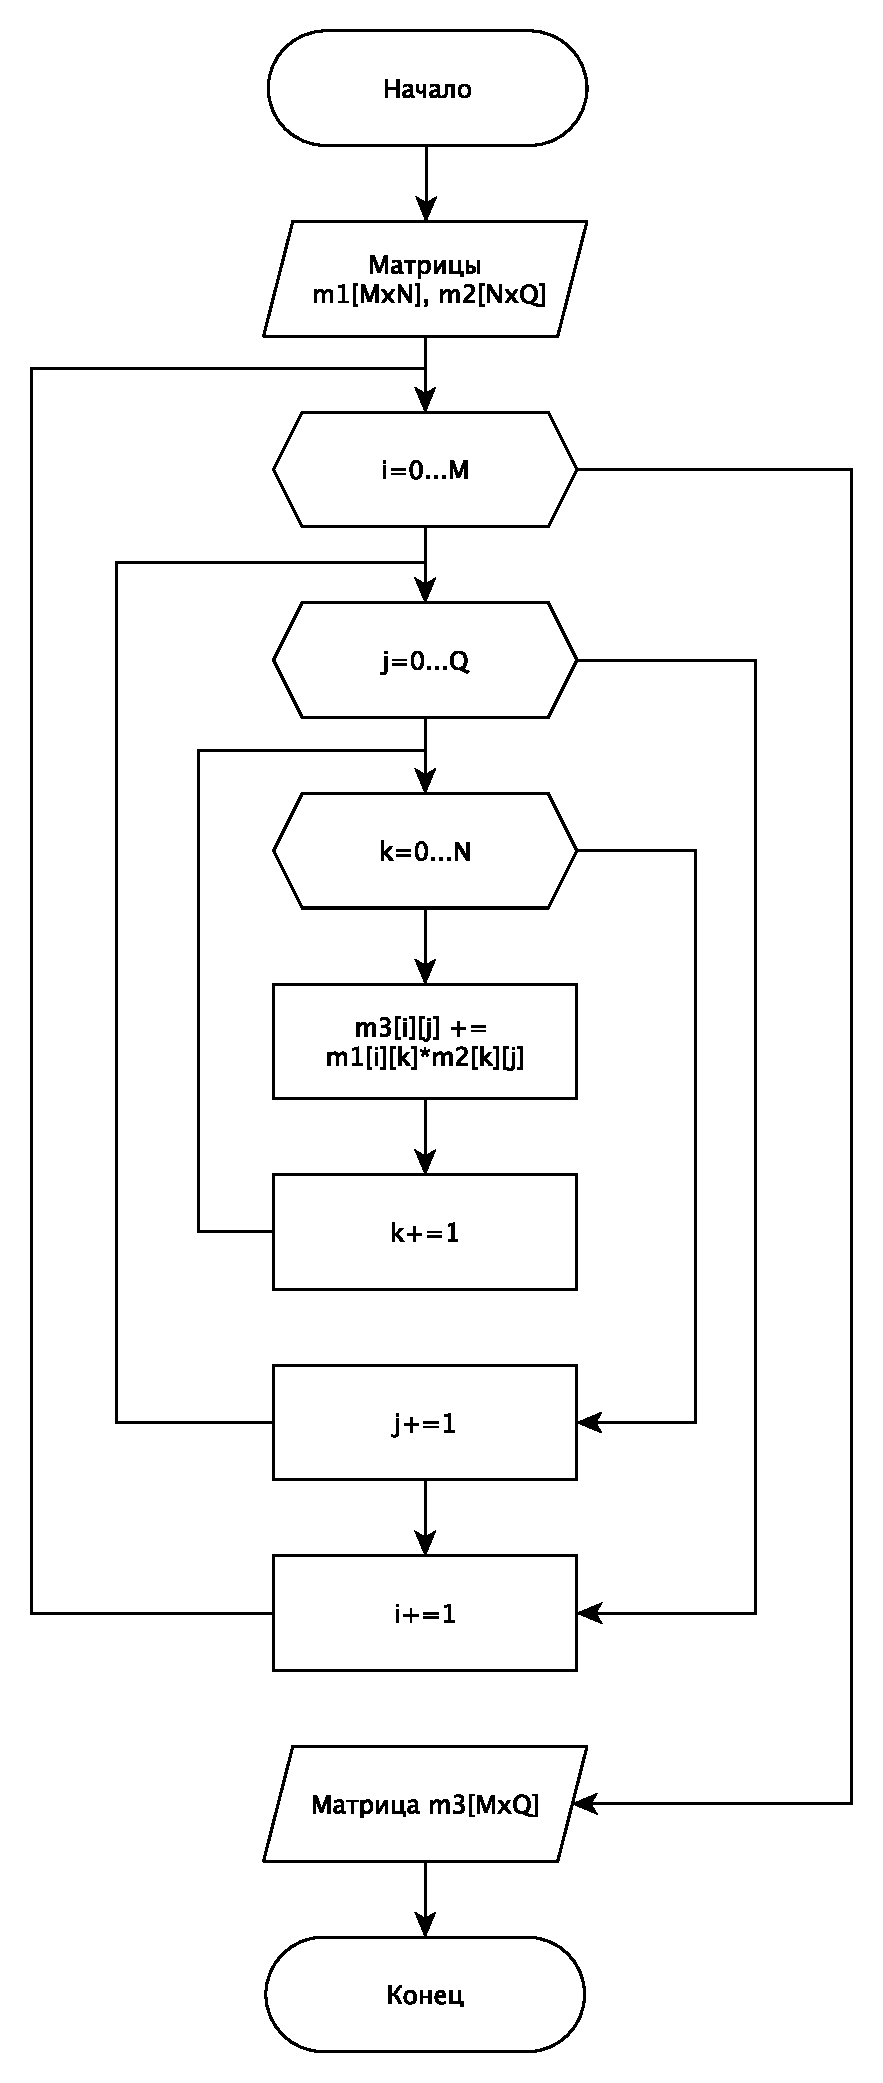
\includegraphics[scale=0.5]{shema1.pdf}
\caption{Алгоритм стандартного произведения матриц}
\end{figure}

\subsection{Алгоритм Винограда}
На рисунке 2.3 представлен алгоритм Винограда для перемножения матриц.
\begin{figure}
\centering
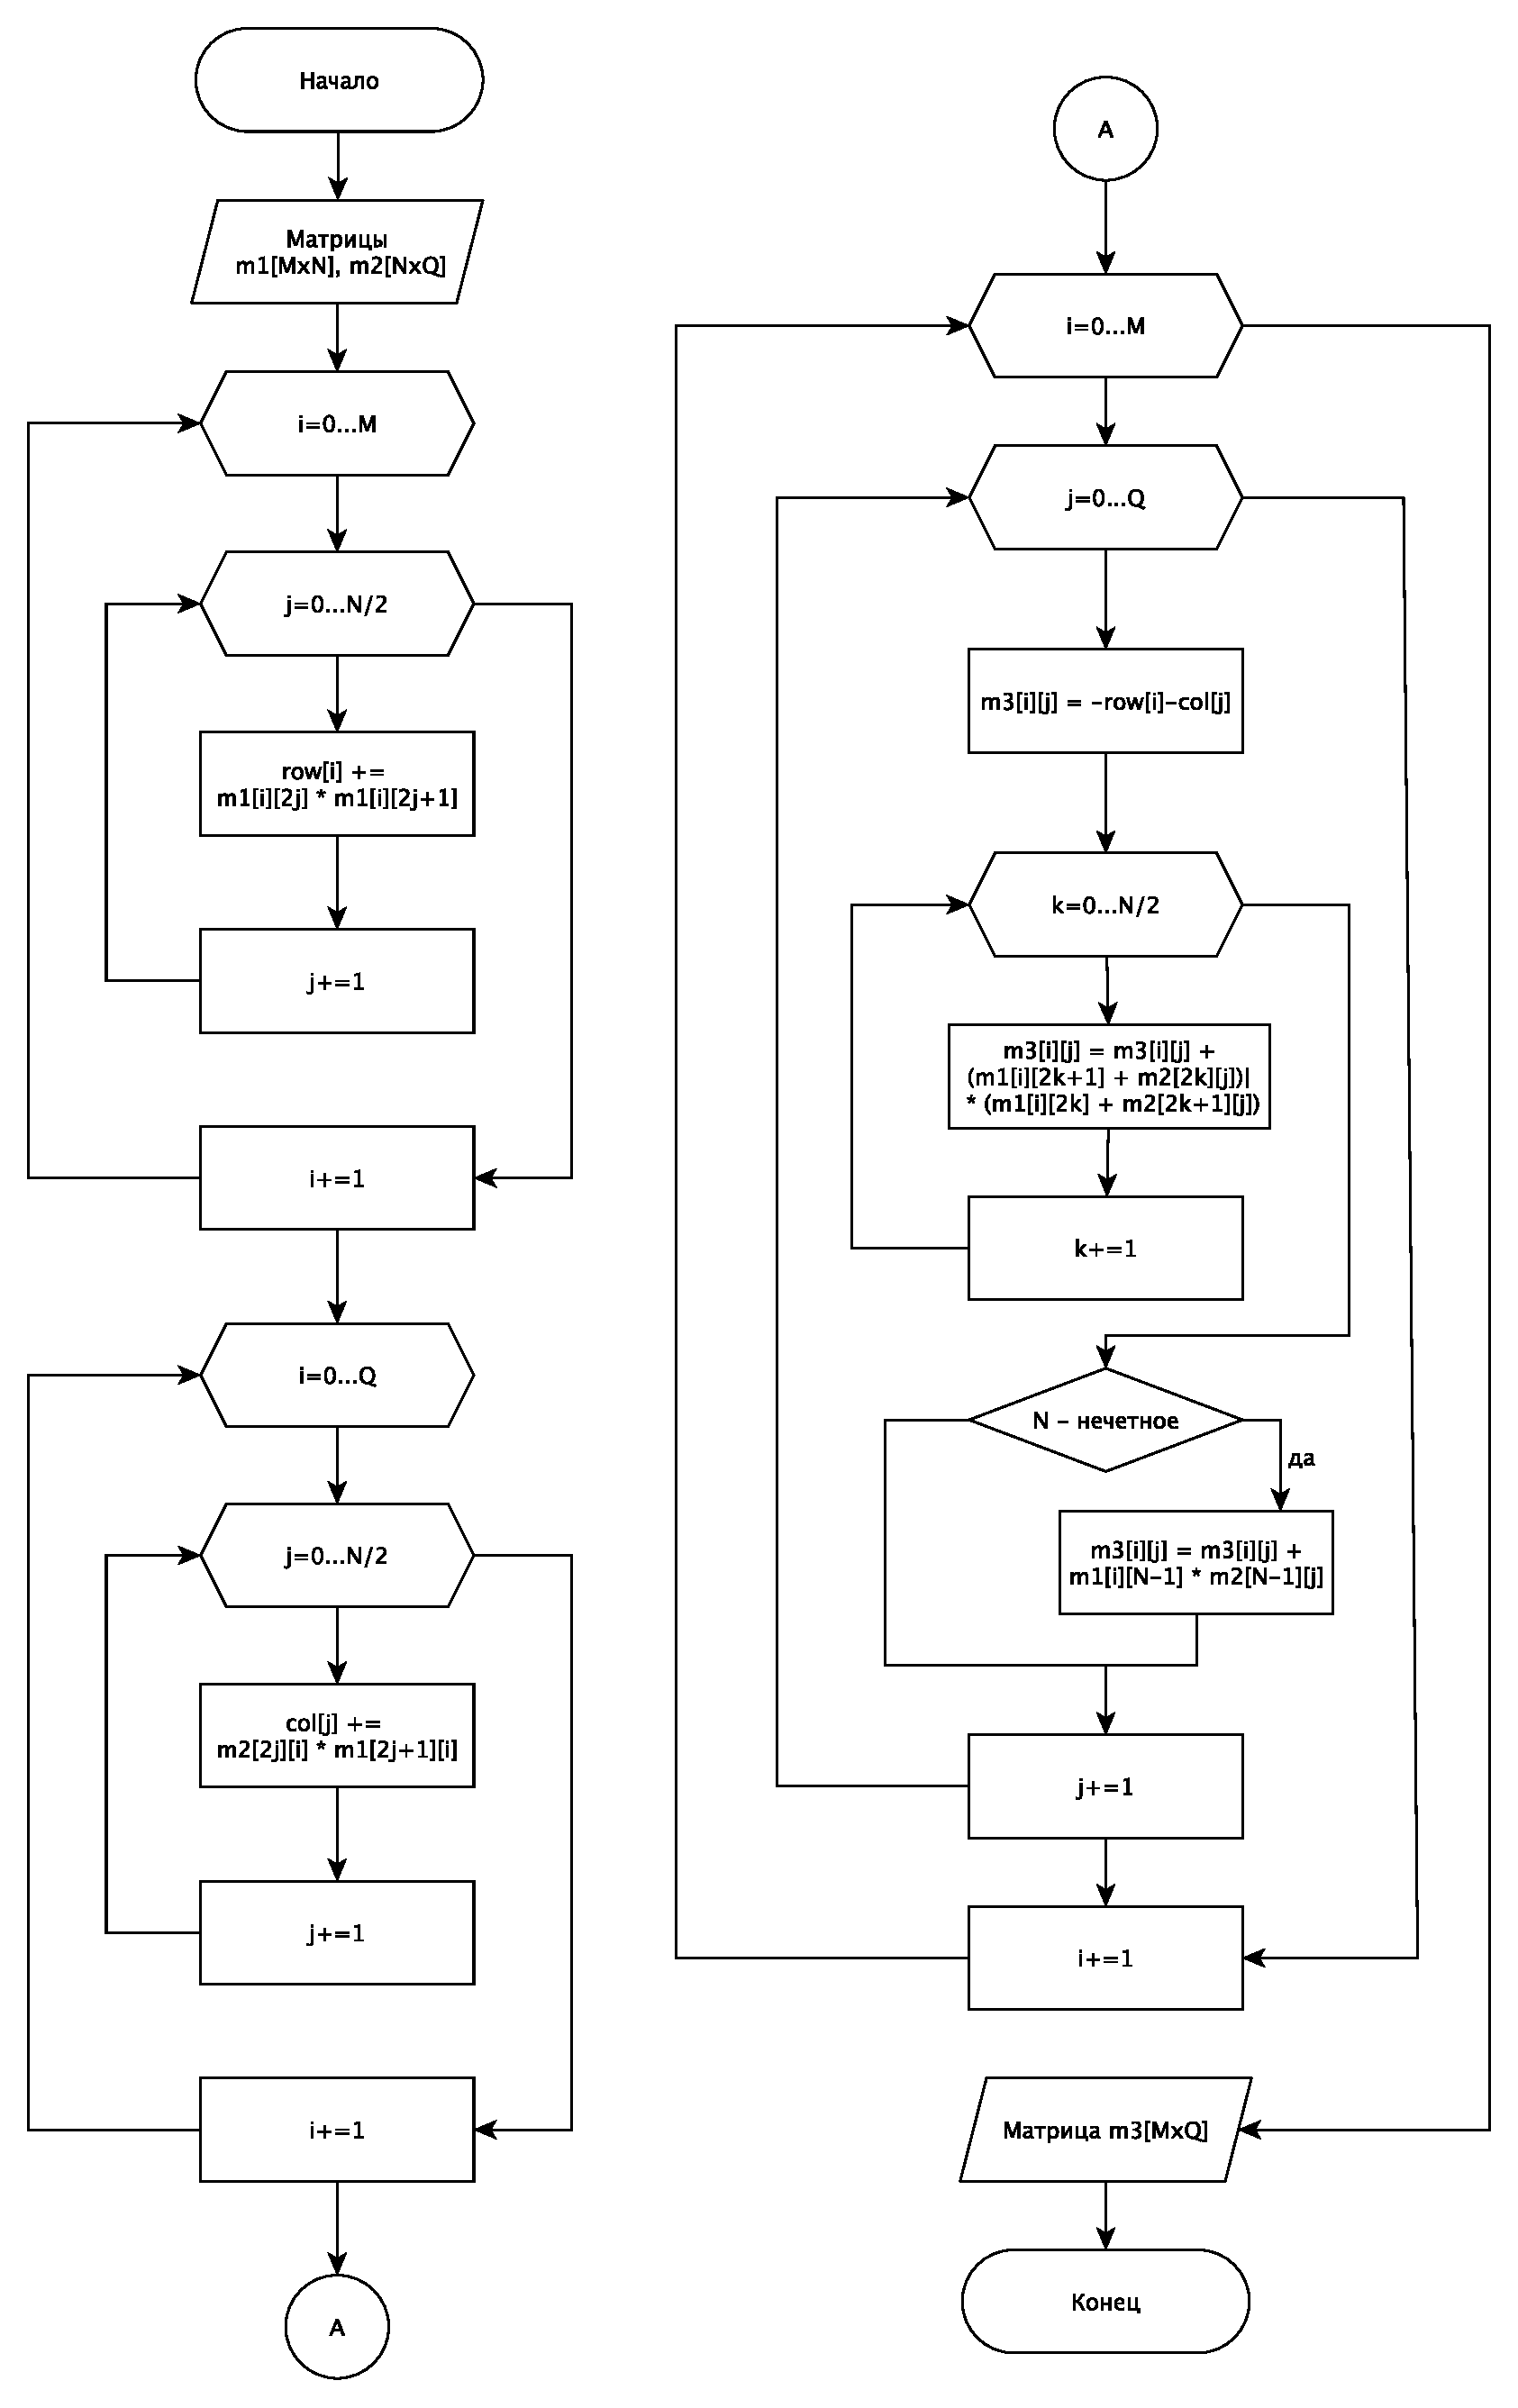
\includegraphics[scale=0.41]{shema2.pdf}
\caption{Алгоритм Винограда}
\end{figure}

\subsection{Алгоритм Винограда с оптимизациями}
На рисунке 2.4 представлен алгоритм Винограда c оптимизациями.
\begin{figure}
\centering
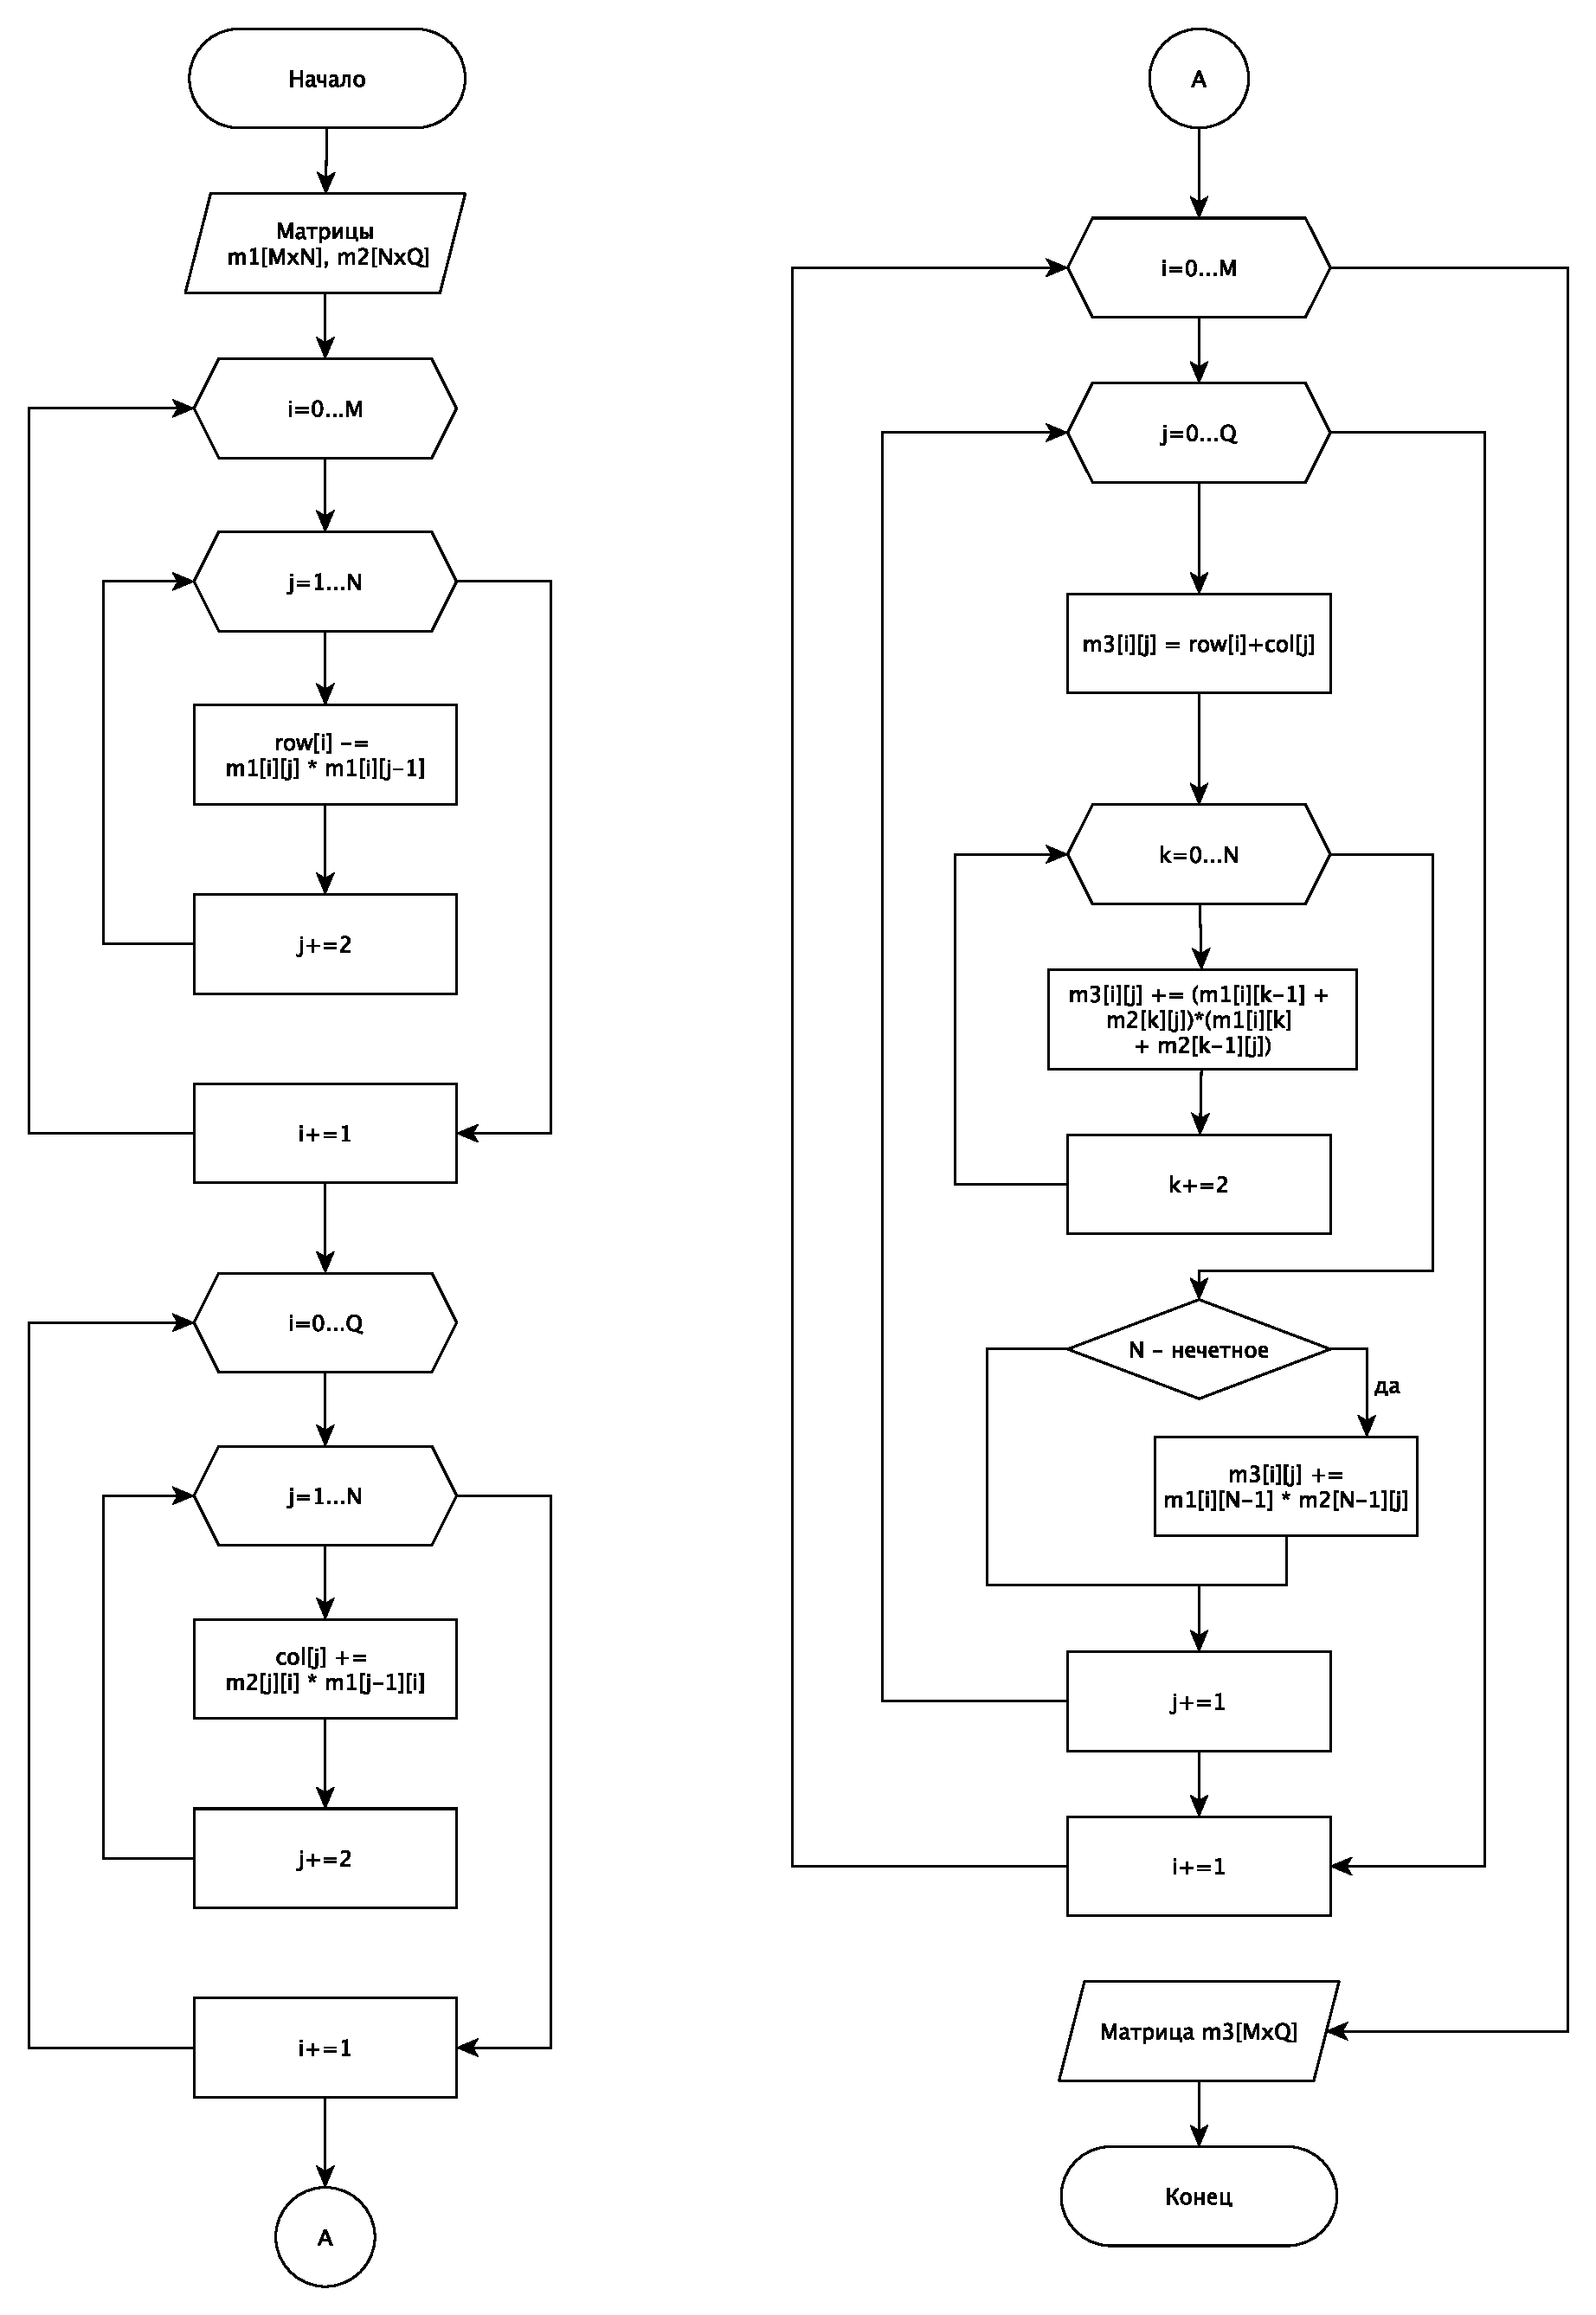
\includegraphics[scale=0.41]{shema3.pdf}
\caption{Оптимизированный алгоритм Винограда}
\end{figure}

\section{Сравнительный анализ алгоритмов}
Произведем теоретическую оценку трудоемкости алгоритмов умножения матриц.
\subsection{Стандартный алгоритм}
		$$f=2+M(2+2+Q(2+2+N(2+8+1+1+1)))=13MNQ+4MQ+4M+2$$
		Оценка трудоемкости приближается к наиболее растущим слагаемым, здесь куб линейного размера матриц. 
\subsection{Алгоритм Винограда}
		
		Предназначен для снижения доли умножения
		
		$$c_{ij}=\underbrace{u_1u_2u_3u_4}_{\vec{u}}*
		\underbrace{\begin{pmatrix} 
    			v_1 \\
   			v_2 \\ 
   			v_3 \\ 
    			v_4
  		\end{pmatrix}}_{\vec{v}}=u_1v_1+u_2v_2+u_3v_3+u_4v_4=(u_1+v_2)(u_2+v_1)+(u_3+v_4)(u_4+v_3)-\underbrace{u_1u_2-u_3u_4-v_1v_2-v_3v_4}_{\text{Вычисляется заранее для строк}}
		$$
		Таким образом, трудоемкость:
		$$f=2+M(2+2+Q(2+4+3+3+N/2(3+12+11)))=13MNQ+12MQ+4M+2$$
		
		Доля умножения меньше чем в стандартном. 
		
        \subsection{Алгоритм Винограда с соответствующими оптимизациями}
		
		 Введем оптимизации: 
		 \begin{enumerate}
		 	\item+=
			\item j<N, j+=2 
			\item Считаем суммы уже отрицательными
		\end{enumerate}
		
		Тогда трудоемкость:
		$$f=2+M(2+2+Q(2+6+2+N/2(2+3+7+6)))=9MNQ+10MQ+4M+2$$
		
		Доля умножения меньше чем в стандартном. 

\subsection{Вывод}
На основе вышеприведенного анализа можно сделать вывод о том, что предварительная обработка в алгоритме Винограда позволяет уменьшить время работы алгоритма.
